\documentclass[a4paper, 10pt]{article}
\usepackage[utf8]{inputenc}
\usepackage[spanish]{babel}
\usepackage{graphicx}
\usepackage{geometry}
\usepackage{listings}
\usepackage{amsmath}
\usepackage{amsfonts}
\usepackage{amssymb}
\usepackage{caratula}

\newcommand{\Z}{\mathbb{Z}}
\def\code#1{\texttt{#1}}
\newcommand\tab[1][0.5cm]{\hspace*{#1}}

\geometry{a4paper, margin=0.7in}

\begin{document}
    %Caratula
    \pagenumbering{gobble}
    \newpage

    \begin{center}
        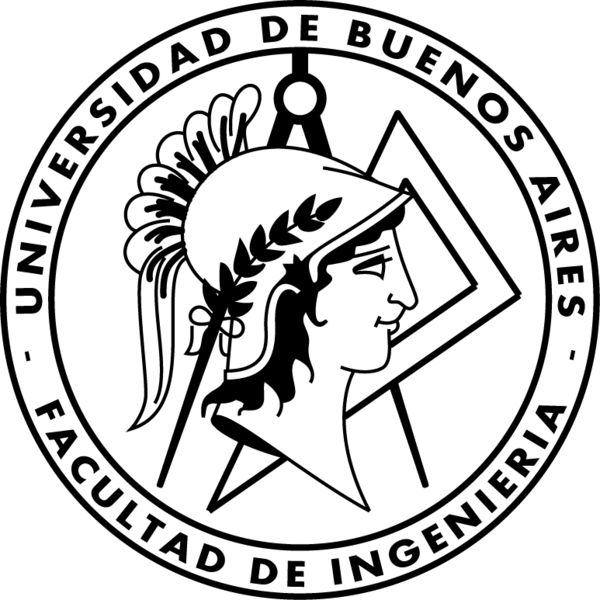
\includegraphics{images/logo}
    \end{center}

    \materia{Teoría de Algoritmos 2}
    \submateria{Segundo Cuatrimestre 2017}
    \titulo{Trabajo Práctico 1}

    \integrante{Rodrigo De Rosa}{97799}{rodrigoderosa@outlook.com}
    \integrante{Marcos Schapira}{97934}{schapiramarcos@gmail.com}
    \integrante{Facundo Guerrero}{97981}{facundoiguerrero@gmail.com}
    \maketitle
    %Fin caratula
    %Table of contents
    \newpage
    \pagenumbering{roman}
    \tableofcontents
    %Fin table of contents
    %Informe
    \newpage
	\pagenumbering{arabic}
	
	\section{Colussi}
		
		\emph{Algoritmo de Livio Colussi 1991} \\
		
		\tab Este algoritmo surge como una optimización del algoritmo de Knuth, Morris y Pratt (que a su vez es una
   		optimización del de Morris y Pratt, que a su vez es una optimización del algoritmo ingenuo).
		
		\subsection{Funcionamiento}    		
    			La idea del algoritmo es identificar \emph{holes} y \emph{no-holes} en el patrón para poder comparar al mismo con el texto
    			en busca de matches es dos pasos. \\
    			\tab Los \emph{holes} son aquellos cuyo valor de kmpNext (del algoritmo KMP) es -1 y los \emph{no-holes} aquellos cuyo 
    			valor de kmpNext es distinto de -1. \\
    			\tab Cada intento del algoritmo consiste entonces de dos pasos:
    			\begin{enumerate}
    				\item Se compara de izquierda a derecha, comparando sólo las posiciones que corresponden a 'no huecos' con los
        			caracteres del texto que corresponden a sus respectivas posiciones.
        			\item Se compara de derecha a izquierda, comparando sóllo las posiciones que corresponden a \emph{holes}.
    			\end{enumerate}
			\tab Esta estrategia tiene las siguientes ventajas:
			\begin{itemize}
				\item Si hay un mismatch en la primera fase, luego de un correcto desplazamiento, no será necesario comparar a 
        			los caracteres del patrón que son 'no huecos' con los caracteres del texto que están en el mismo lugar.
        		\end{itemize}
        		\begin{center}
        			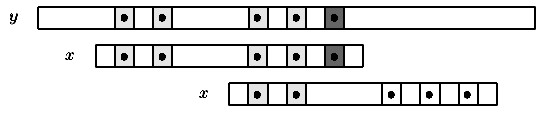
\includegraphics[width=4.25in, height=1in]{images/nohole}
        			\\ En este caso hay un mismatch en un \emph{no-hole}. En esta situación, no es necesario comparar los dos primeros
			    \emph{no-hole} del patrón luego del desplazamiento
		    \end{center}
        		\begin{itemize}
        			\item Si hay un mismatch en la segunda fase, entonces hay un sufijo del patrón que es igual a un factor del texto
        			y luego de desplazar correctamente estos seguirán coincidiendo y no es necesario volver a compararlos.
			\end{itemize}
			\begin{center}
        			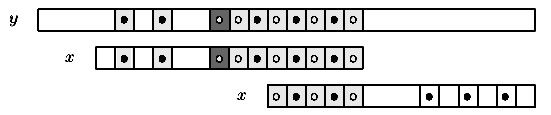
\includegraphics[width=4.25in, height=1in]{images/hole}
				\\En este caso, luego del shift, no hace falta comparar el prefijo que coincidió.
		    \end{center}
		\subsection{Implementación}
			Para la implementación de este algoritmo, se utiliza una serie de \emph{tablas} (implementadas como listas) para el
			preprocesamiento del patrón a buscar. Dichas tablas permiten realizar desplazamientos en el texto durante la comparación
			asegurándonos que no nos perderemos de nada y asegurándonos una mayor performance. \\
			\tab Dichas tablas son: \\ \\
			\tab\tab Kmin[$i$] = $\left\{ 
					\begin{array}{lcc}
             			d &   sii  & x[0 ... i - d - 1] = x[d ... i - 1] \wedge x[i - d] = x[i] \\
             			\\ 0 & sino
    					\end{array}
 		 		  \right.$
 		 	\\ \tab Esta tabla indica el shift que se debe realizar en caso de que la posición $i$ pertenezca a un \emph{no-hole}. \\
 		 	\tab\tab Rmin[$i$] = es el equivalente a Kmin pero para los \emph{hole}. \\
 		 	\tab Sea $ND + 1$ la cantidad de \emph{no-holes} en el patrón x, la tabla $h$ contiene a todos los \emph{no-holes} de
 		 	menor a mayor y luego a los $m - ND - 1$ \emph{holes} en orden decreciente. Esto es para recorrer a los \emph{no-holes}
 		 	de izquierda a derecha y a los \emph{holes} de derecha a izquierda. \\ \\
 		 	\tab\tab h[$i$] = $\left\{ 
					\begin{array}{lcc}
             			h[i] < h[i+1] (no-hole) &   si  & i \in [0, ND)\\
             			\\ h[i] > h[i+1] (hole) & si & i \in [ND, m)
    					\end{array}
 		 		  \right.$
 		 	\\ \\ \tab\tab first[$u$] = $v$, con $v$ entero más pequeño tal que $u \leq h[v]$. 
 		 	\\\\ \tab Para calcular el valor de Kmin, utilizamos la tabla hmax:
 		 	\\ \tab\tab hmax[$i$] es tal que: $\left\{ 
					\begin{array}{lcc}
             			x[i ... hmax[i] - 1] = x[0 ... hmax[i] - i -1]\\
             			\\ x[hmax[i]] \neq x[hmax[i] - i]
    					\end{array}
 		 		  \right.$
 		 	\\\\ \tab Finalmente, utilizamos la tabla \\
 		 	\tab\tab nhd0[$i$] = cantidad de \emph{no-holes} hasta la posición $i$. \\ \\
 		 	\tab Con estas tablas, armamos las dos tablas que realmente utilizamos en el algoritmo: \emph{shift} y \emph{next}. El
 		 	valor de ambas depende de si la posición $i$ contiene a un \emph{hole} o un \emph{no-hole} y se definen como:
 		 	\\ \tab\tab shift[$i$] = $\left\{ 
					\begin{array}{lcc}
             			kmin[h[i]] & si & i \in [0, ND)\\
             			\\ rmin[h[i]] & si & i \in [0, ND)
    					\end{array}
 		 		  \right.$
 		 	\\ \tab\tab next[$i$] = $\left\{ 
					\begin{array}{lcc}
             			ndh0[h[i] - kmin[h[i]]] & si & i \in [0, ND)\\
             			\\ ndh0[m - rmin[h[i]]] & si & i \in [0, ND)
    					\end{array}
 		 		  \right.$
 		 	\\ \tab Por lo tanto, si la ventana está ubicada en $T[j ... j + m - 1]$, cuando hay un mismatch entre $P[h[r]]$ y 
 		 	$T[j + h[r]]$, la ventana debe ser desplazada en \emph{shift[$r$]} y las comparaciones iniciarán desde la posición
 		 	\emph{h[next[$r$]]} del patrón. \\
 		 	\tab Por último, devolveremos un match sólo en dos casos:
 		 	\begin{itemize}
 		 		\item Si $i = m$.Arrancamos de $i=0$ y llegamos al final sin errores.
        			\item Si $j + m - 1 = j + h[i]$. Este es el caso en el que la comparación no empieza desde el inicio de P gracias
                 a algún dato del preprocessing y h[i] = m-1, es decir, llegamos al final de las comparaciones.
 		 	\end{itemize}
		
		\subsection{Complejidad}
			La complejidad de este algoritmo es $O(n + m)$, siendo $O(m)$ la etapa de preprocesamiento y $O(n)$ la etapa de búsqueda.
			En el peor de los casos, realiza $\frac{3}{2}n$ comparaciones, con $n$ la cantidad de caracteres del \emph{Texto} y $m$
			la cantidad de caracteres del \emph{Patrón}.
		
		\subsection{Características del algoritmo y casos de prueba}
			Este algoritmo tiene una característica importante y es que no es necesario conocer el alfabeto para buscar matches, pues
			en ningún momento es necesario conocer al mismo para ninguna de las tareas que se realizan en el mismo. \\
			\tab Es importante destacar que, si bien fue concebido como una mejora de KMP, en la mayoría de las pruebas que realizamos
			comparando el algoritmo ingenuo, MP, KMP y Colussi, este último fue el de peor performance. En el único caso en el que
			logramos que Colussi fuera el mejor fue un caso en el que teníamos un texto de la forma: \\
			\begin{verbatim}
			aaaaaaaaaaa#aaaaaaaaaaaaaa#aaaaaaaaaaa#....
			123456789#123456789#123456789#123456789#.....
			aaa..
			123..
			\end{verbatim}		
			\tab Con un patrón de la forma:
			\begin{verbatim}
			aaaaaaa#aaaaaa
			\end{verbatim}
			\tab En este caso, Colussi fue mucho mejor que los otros algoritmos previamente mencionados (aproximadamente un $50\%$ 
			mejor). Pero en todo el resto (archivos de ADN, textos en español, textos en inglés, código en C) tanto con texto largo
			y patrón corto como con texto corto y patrón largo, encontramos que este algoritmo no tuvo la performance esperada, siendo
			superado incluso por el algoritmo ingenuo.
\end{document}
